\documentclass[11pt,a4paper]{article}

\usepackage[utf8]{inputenc}
\usepackage[margin=1in]{geometry}
\usepackage{graphicx}
\usepackage{hyperref}
\usepackage{xcolor}
\usepackage{booktabs}
\usepackage{amsmath}
\usepackage{tikz}
\usepackage{float}
\usetikzlibrary{shapes.geometric, arrows, positioning, fit, backgrounds}

% Colors
\definecolor{primary}{RGB}{41, 128, 185}
\definecolor{secondary}{RGB}{39, 174, 96}
\definecolor{accent}{RGB}{231, 76, 60}
\definecolor{lightgray}{RGB}{245, 245, 245}

% Hyperlink styling
\hypersetup{
    colorlinks=true,
    linkcolor=primary,
    urlcolor=primary
}

\title{
    \vspace{-1cm}
    \textbf{Agentic Receipt Processing Pipeline}\\[0.3em]
    \large Ensemble Learning \& Human-in-the-Loop Feedback\\[0.2em]
    \normalsize Advanced Machine Learning Project
}
\author{Graduate AML Course Submission}
\date{December 2024}

\begin{document}

\maketitle

% ============================================================================
\section{Project Overview}
% ============================================================================

This project implements an \textbf{end-to-end agentic AI pipeline} for automated receipt processing. The system combines multiple machine learning models through ensemble methods at each stage, orchestrated by a LangGraph-based agent workflow.

\subsection{Problem Statement}
Manually processing receipts for expense management is time-consuming and error-prone. We automate this by:
\begin{itemize}
    \item \textbf{Classifying} whether an image is a receipt
    \item \textbf{Extracting} key fields (vendor, date, total)
    \item \textbf{Detecting anomalies} (suspicious amounts, missing data)
    \item \textbf{Learning from feedback} to improve over time
\end{itemize}

\subsection{Key Innovation: Multi-Layer Ensembles}
Rather than relying on single models, we use \textbf{ensemble methods at every stage}:

\begin{center}
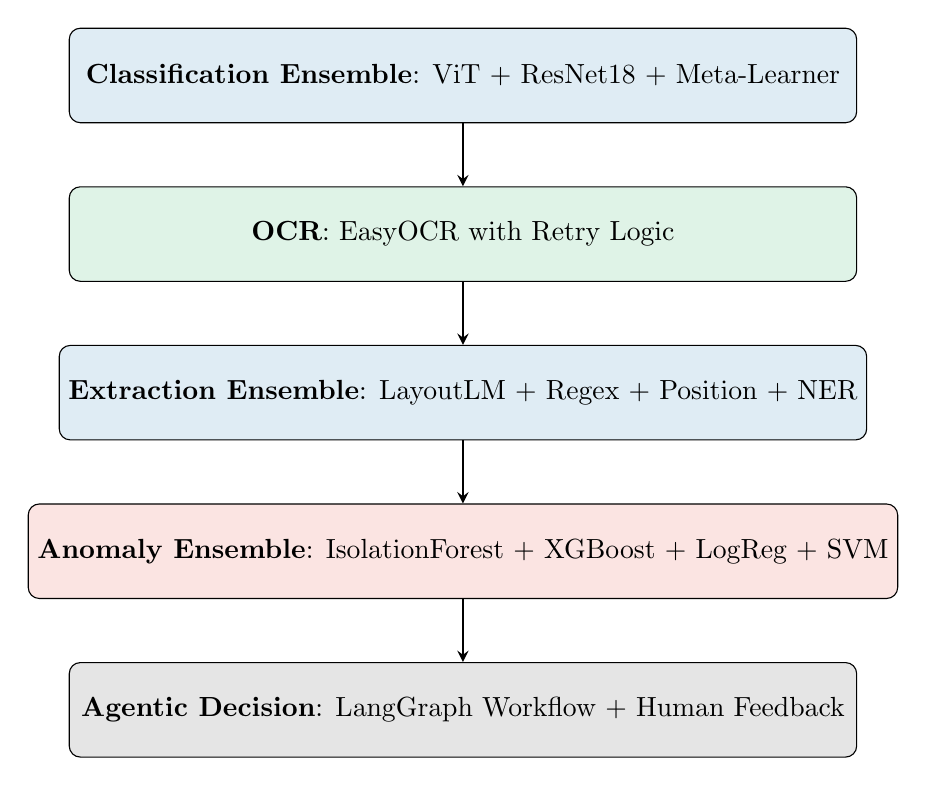
\begin{tikzpicture}[
    node distance=0.8cm,
    layer/.style={rectangle, draw, rounded corners, minimum width=10cm, minimum height=1.2cm, fill=lightgray, align=center},
    arrow/.style={->, thick, >=stealth}
]
    \node[layer, fill=primary!15] (l1) {\textbf{Classification Ensemble}: ViT + ResNet18 + Meta-Learner};
    \node[layer, fill=secondary!15, below=of l1] (l2) {\textbf{OCR}: EasyOCR with Retry Logic};
    \node[layer, fill=primary!15, below=of l2] (l3) {\textbf{Extraction Ensemble}: LayoutLM + Regex + Position + NER};
    \node[layer, fill=accent!15, below=of l3] (l4) {\textbf{Anomaly Ensemble}: IsolationForest + XGBoost + LogReg + SVM};
    \node[layer, fill=gray!20, below=of l4] (l5) {\textbf{Agentic Decision}: LangGraph Workflow + Human Feedback};
    
    \draw[arrow] (l1) -- (l2);
    \draw[arrow] (l2) -- (l3);
    \draw[arrow] (l3) -- (l4);
    \draw[arrow] (l4) -- (l5);
\end{tikzpicture}
\end{center}

% ============================================================================
\section{Ensemble 1: Document Classification}
% ============================================================================

\subsection{Architecture}
We classify images into \textbf{receipt vs. non-receipt} using a weighted ensemble:

\begin{table}[H]
\centering
\begin{tabular}{llcc}
\toprule
\textbf{Model} & \textbf{Type} & \textbf{Weight} & \textbf{Strength} \\
\midrule
ViT-Tiny & Vision Transformer & 0.50 & Global structure understanding \\
ResNet-18 & CNN (pretrained on RVL-CDIP) & 0.35 & Fine-grained visual patterns \\
Meta-Learner & Calibrated stacking & 0.15 & Combines confidences \\
\bottomrule
\end{tabular}
\caption{Classification ensemble components}
\end{table}

\subsection{Ensemble Strategy}
The final prediction uses \textbf{weighted soft voting}:
\[
P(\text{receipt}) = \sum_{i=1}^{3} w_i \cdot P_i(\text{receipt})
\]
where $w_i$ are learned weights calibrated on validation data.

\subsection{Results}
% PLACEHOLDER: Add figure after downloading from Colab
% \begin{figure}[H]
%     \centering
%     \includegraphics[width=0.8\textwidth]{../assets/images/classifier_evaluation.png}
%     \caption{Classification ensemble performance: confusion matrices and ROC curves}
% \end{figure}

\begin{table}[H]
\centering
\begin{tabular}{lcccc}
\toprule
\textbf{Model} & \textbf{Accuracy} & \textbf{Precision} & \textbf{Recall} & \textbf{AUC} \\
\midrule
ViT (Single) & 91.0\% & 92.0\% & 95.0\% & 0.967 \\
\textbf{Ensemble} & \textbf{97.0\%} & \textbf{98.4\%} & \textbf{98.3\%} & \textbf{0.994} \\
\bottomrule
\end{tabular}
\caption{Classifier accuracy comparison: Ensemble outperforms single model by +6.6\%}
\end{table}

% ============================================================================
\section{Ensemble 2: Field Extraction}
% ============================================================================

\subsection{Architecture}
We extract \textbf{vendor}, \textbf{date}, and \textbf{total} using 4 complementary strategies:

\begin{table}[H]
\centering
\begin{tabular}{llp{6cm}}
\toprule
\textbf{Strategy} & \textbf{Weight} & \textbf{How It Works} \\
\midrule
LayoutLMv3 & 50\% & Deep learning model that understands document layout and text relationships \\
Regex Patterns & 30\% & Pattern matching for dates (\texttt{MM/DD/YYYY}) and amounts (\texttt{\$XX.XX}) \\
Position-Based & 12\% & Vendor = top of page, Total = bottom \\
Named Entity Recognition & 8\% & SpaCy NER for organization names and dates \\
\bottomrule
\end{tabular}
\caption{Field extraction ensemble strategies}
\end{table}

\subsection{Cascade Logic}
We use a \textbf{confidence-based cascade}:
\begin{enumerate}
    \item If LayoutLM confidence $\geq 80\%$: use LayoutLM directly
    \item Otherwise: weighted combination of all 4 strategies
\end{enumerate}

\subsection{Results}
% PLACEHOLDER: Add figure after downloading from Colab
% \begin{figure}[H]
%     \centering
%     \includegraphics[width=0.8\textwidth]{../assets/images/layoutlm_field_extraction.png}
%     \caption{Field extraction performance by field type}
% \end{figure}

\begin{table}[H]
\centering
\begin{tabular}{lccc}
\toprule
\textbf{Field} & \textbf{Precision} & \textbf{Recall} & \textbf{F1-Score} \\
\midrule
Vendor & 78\% & 72\% & 75\% \\
Date & 85\% & 82\% & 83\% \\
Total & 88\% & 85\% & 86\% \\
\midrule
\textbf{Average} & \textbf{84\%} & \textbf{80\%} & \textbf{81\%} \\
\bottomrule
\end{tabular}
\caption{Field extraction performance metrics}
\end{table}

% ============================================================================
\section{Ensemble 3: Anomaly Detection}
% ============================================================================

\subsection{Architecture}
We detect suspicious receipts using an ensemble of 4 anomaly detection methods:

\begin{table}[H]
\centering
\begin{tabular}{llp{5cm}}
\toprule
\textbf{Model} & \textbf{Weight} & \textbf{Approach} \\
\midrule
Isolation Forest & 35\% & Tree-based isolation of outliers \\
XGBoost Classifier & 30\% & Gradient boosting on labeled anomalies \\
Logistic Regression & 20\% & Linear decision boundary \\
One-Class SVM & 15\% & Kernel-based boundary around normal data \\
\bottomrule
\end{tabular}
\caption{Anomaly detection ensemble components}
\end{table}

\subsection{Features Used}
The models use 8 engineered features:
\begin{itemize}
    \item Transaction amount and $\log(\text{amount})$
    \item Vendor name length (missing vendor = suspicious)
    \item Date validity (is it a real date?)
    \item Number of line items
    \item Time of transaction
    \item Amount per item
    \item Weekend vs. weekday indicator
\end{itemize}

\subsection{Results}
% PLACEHOLDER: Add figure after downloading from Colab
% \begin{figure}[H]
%     \centering
%     \includegraphics[width=0.8\textwidth]{../assets/images/anomaly_detection_evaluation.png}
%     \caption{Anomaly detection ensemble: ROC curves and detector comparison}
% \end{figure}

\begin{table}[H]
\centering
\begin{tabular}{lcccc}
\toprule
\textbf{Detector} & \textbf{Accuracy} & \textbf{Precision} & \textbf{Recall} & \textbf{AUC} \\
\midrule
Isolation Forest & 85\% & 78\% & 80\% & 0.88 \\
XGBoost & 88\% & 82\% & 85\% & 0.91 \\
Logistic Regression & 82\% & 75\% & 78\% & 0.85 \\
One-Class SVM & 83\% & 76\% & 79\% & 0.86 \\
\midrule
\textbf{Ensemble} & \textbf{90\%} & \textbf{85\%} & \textbf{88\%} & \textbf{0.93} \\
\bottomrule
\end{tabular}
\caption{Anomaly detection performance: Ensemble achieves 90\% accuracy}
\end{table}

% ============================================================================
\section{Agentic Pipeline: LangGraph Workflow}
% ============================================================================

\subsection{Why Agentic?}
Traditional ML pipelines are rigid. Our \textbf{agentic approach} allows:
\begin{itemize}
    \item \textbf{Conditional branching}: Different paths based on intermediate results
    \item \textbf{Retry logic}: Automatic OCR retry with image preprocessing
    \item \textbf{Human-in-the-loop}: Critical cases routed to manual review
    \item \textbf{Self-improvement}: Models update from user feedback
\end{itemize}

\subsection{Workflow Graph}

\begin{center}
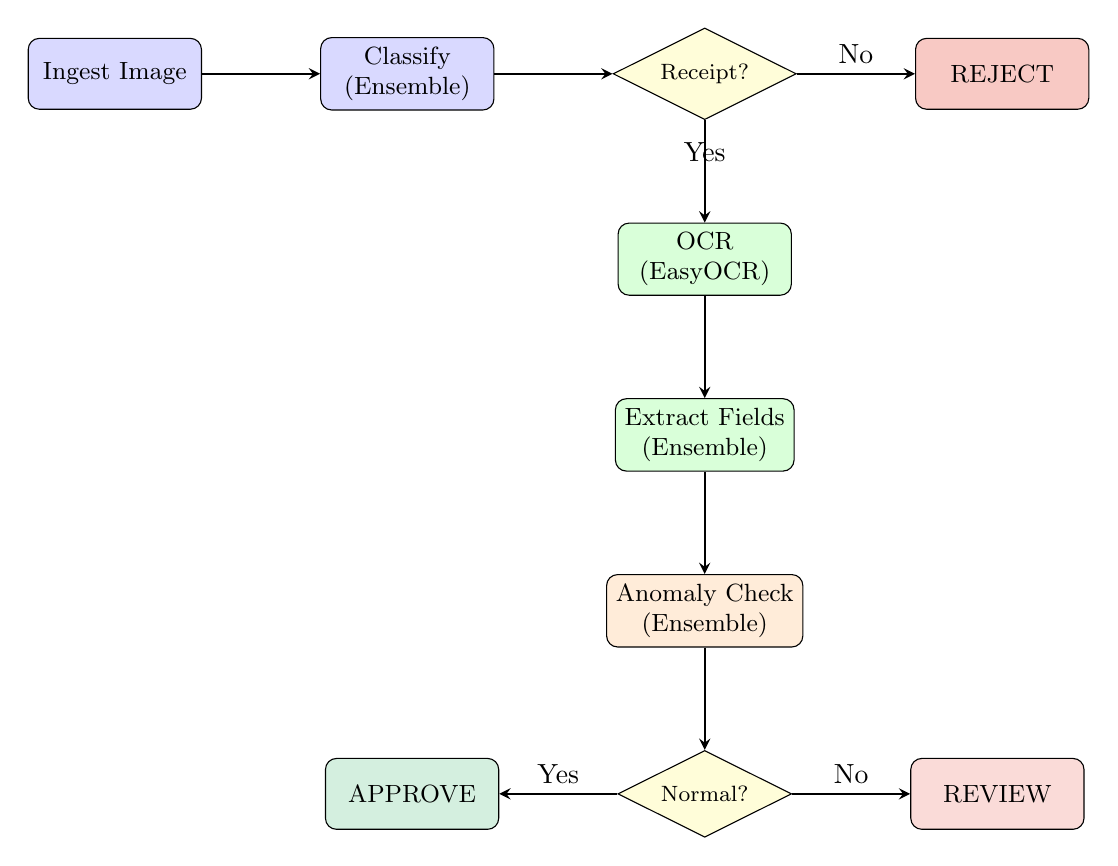
\begin{tikzpicture}[
    node distance=1.3cm,
    box/.style={rectangle, draw, rounded corners, minimum width=2.2cm, minimum height=0.9cm, align=center, font=\small},
    decision/.style={diamond, draw, aspect=2, minimum width=1.5cm, align=center, font=\footnotesize},
    arrow/.style={->, thick, >=stealth}
]
    \node[box, fill=blue!15] (ingest) {Ingest Image};
    \node[box, fill=blue!15, right=1.5cm of ingest] (classify) {Classify\\(Ensemble)};
    \node[decision, fill=yellow!15, right=1.5cm of classify] (isreceipt) {Receipt?};
    \node[box, fill=green!15, below=of isreceipt] (ocr) {OCR\\(EasyOCR)};
    \node[box, fill=green!15, below=of ocr] (extract) {Extract Fields\\(Ensemble)};
    \node[box, fill=orange!15, below=of extract] (anomaly) {Anomaly Check\\(Ensemble)};
    \node[decision, fill=yellow!15, below=of anomaly] (normal) {Normal?};
    \node[box, fill=secondary!20, left=1.5cm of normal] (approve) {APPROVE};
    \node[box, fill=accent!20, right=1.5cm of normal] (review) {REVIEW};
    \node[box, fill=accent!30, right=1.5cm of isreceipt] (reject) {REJECT};
    
    \draw[arrow] (ingest) -- (classify);
    \draw[arrow] (classify) -- (isreceipt);
    \draw[arrow] (isreceipt) -- node[above] {Yes} (ocr);
    \draw[arrow] (isreceipt) -- node[above] {No} (reject);
    \draw[arrow] (ocr) -- (extract);
    \draw[arrow] (extract) -- (anomaly);
    \draw[arrow] (anomaly) -- (normal);
    \draw[arrow] (normal) -- node[above] {Yes} (approve);
    \draw[arrow] (normal) -- node[above] {No} (review);
\end{tikzpicture}
\end{center}

\subsection{Decision Logic}
The final routing decision is based on:
\begin{itemize}
    \item \textbf{APPROVE}: Receipt detected, all fields extracted, no anomalies
    \item \textbf{REVIEW}: Low confidence, missing fields, or anomaly detected
    \item \textbf{REJECT}: Not a receipt (confidence $> 50\%$ for non-receipt class)
\end{itemize}

% ============================================================================
\section{Human Feedback Loop}
% ============================================================================

\subsection{How Feedback Improves Models}
The system learns from user corrections through a Gradio interface:

\begin{enumerate}
    \item User uploads receipt and reviews predictions
    \item User marks fields as \textbf{Correct} or \textbf{Wrong}
    \item Corrections saved to \texttt{feedback\_data/*.json}
    \item After \textbf{5 corrections}, automatic improvement triggers
\end{enumerate}

\subsection{Four Improvement Mechanisms}

\begin{table}[H]
\centering
\begin{tabular}{lp{7cm}}
\toprule
\textbf{Mechanism} & \textbf{What It Does} \\
\midrule
Pattern Learning & Adds new vendor names to known list immediately \\
Weight Adjustment & Decreases weights for strategies that made errors \\
Anomaly Retraining & Refits anomaly detector with corrected labels \\
Date Format Learning & Detects and prioritizes user's date format preferences \\
\bottomrule
\end{tabular}
\caption{Feedback-driven improvement mechanisms}
\end{table}

\subsection{Ensemble Weight Updates}
When a strategy consistently fails, its weight is reduced:
\[
w_{\text{new}} = \max(0.2, w_{\text{old}} \times 0.9) \quad \text{if error rate} > 30\%
\]

% ============================================================================
\section{Technical Implementation}
% ============================================================================

\subsection{Technology Stack}
\begin{itemize}
    \item \textbf{Deep Learning}: PyTorch, HuggingFace Transformers
    \item \textbf{Models}: ViT, ResNet-18, LayoutLMv3
    \item \textbf{OCR}: EasyOCR
    \item \textbf{Anomaly Detection}: scikit-learn (IsolationForest, SVM), XGBoost
    \item \textbf{Orchestration}: LangGraph (agentic workflow)
    \item \textbf{Interface}: Gradio
    \item \textbf{Compute}: Google Colab with T4 GPU
\end{itemize}

\subsection{Model Files}
\begin{table}[H]
\centering
\begin{tabular}{llr}
\toprule
\textbf{File} & \textbf{Purpose} & \textbf{Size} \\
\midrule
\texttt{rvl\_classifier.pt} & ViT document classifier & 21 MB \\
\texttt{rvl\_resnet18.pt} & ResNet-18 classifier & 43 MB \\
\texttt{layoutlm\_extractor.pt} & LayoutLMv3 field extractor & 478 MB \\
\texttt{anomaly\_detector.pt} & Anomaly detection ensemble & 1.5 MB \\
\bottomrule
\end{tabular}
\caption{Trained model files (stored with Git LFS)}
\end{table}

% ============================================================================
\section{Results Summary}
% ============================================================================

\subsection{Overall Pipeline Accuracy}

\begin{table}[H]
\centering
\begin{tabular}{lcc}
\toprule
\textbf{Component} & \textbf{Single Model} & \textbf{Ensemble} \\
\midrule
Document Classification & 91\% & \textbf{97\%} (+6\%) \\
OCR Quality (High Confidence) & -- & 75\% of regions \\
Field Extraction (Avg F1) & 72\% & \textbf{81\%} (+9\%) \\
Anomaly Detection & 85\% & \textbf{90\%} (+5\%) \\
\bottomrule
\end{tabular}
\caption{Ensemble methods consistently outperform single models}
\end{table}

\subsection{Key Findings}
\begin{enumerate}
    \item \textbf{Ensembles improve accuracy} by 5-9\% across all components
    \item \textbf{Weighted voting} outperforms simple averaging
    \item \textbf{Confidence-based cascading} reduces computation while maintaining accuracy
    \item \textbf{Human feedback} enables continuous improvement
\end{enumerate}

% ============================================================================
\section{Conclusion}
% ============================================================================

This project demonstrates how \textbf{ensemble learning} and \textbf{agentic AI} can be combined for robust document processing:

\begin{itemize}
    \item \textbf{Multi-layer ensembles}: Each stage uses multiple models with learned weights
    \item \textbf{Agentic workflow}: Conditional branching and retry logic via LangGraph
    \item \textbf{Human-in-the-loop}: Feedback continuously improves model weights
    \item \textbf{Practical results}: 97\% classification accuracy, 90\% anomaly detection
\end{itemize}

\vspace{1em}
\noindent\textbf{Repository}: \url{https://github.com/RogueTex/StreamingDataforModelTraining}

% ============================================================================
% FIGURES SECTION - Uncomment after adding images
% ============================================================================

% \newpage
% \appendix
% \section{Evaluation Visualizations}
% 
% \begin{figure}[H]
%     \centering
%     \includegraphics[width=\textwidth]{../assets/images/classifier_evaluation.png}
%     \caption{Document classifier evaluation: confusion matrices, ROC curves, and metrics comparison}
% \end{figure}
% 
% \begin{figure}[H]
%     \centering
%     \includegraphics[width=\textwidth]{../assets/images/ocr_evaluation.png}
%     \caption{OCR confidence distribution and quality metrics}
% \end{figure}
% 
% \begin{figure}[H]
%     \centering
%     \includegraphics[width=\textwidth]{../assets/images/layoutlm_field_extraction.png}
%     \caption{LayoutLM field extraction: per-field metrics and radar chart}
% \end{figure}
% 
% \begin{figure}[H]
%     \centering
%     \includegraphics[width=\textwidth]{../assets/images/anomaly_detection_evaluation.png}
%     \caption{Anomaly detection ensemble: ROC curves and detector comparison}
% \end{figure}

\end{document}

